\RequirePackage{amsmath}
\documentclass[twocolumn, times]{aastex631}
\usepackage[spanish,es-minimal,english]{babel}
\usepackage[utf8]{inputenc}
\usepackage{natbib}
%\usepackage{microtype}
\usepackage{hyperref}
\usepackage{savesym}
\savesymbol{tablenum}
\usepackage{siunitx}
\restoresymbol{SIX}{tablenum}
\usepackage[varg]{newtxmath}
\usepackage{newtxtext}
\usepackage{booktabs}
\usepackage{array}   % for \newcolumntype macro
\newcolumntype{L}{>{$}l<{$}} % math-mode version of lrc column types
\newcolumntype{R}{>{$}r<{$}} 
\newcolumntype{C}{>{$}c<{$}} 

\bibliographystyle{aasjournal}

\newcommand\ION[2]{#1\,\scalebox{0.9}[0.8]{\uppercase{#2}}}
\newcounter{ionstage}
\renewcommand{\ion}[2]{\setcounter{ionstage}{#2}% 
  \ensuremath{\mathrm{#1\,\scriptstyle\Roman{ionstage}}}}
\newcommand\hii{\ion{H}{2}}
\newcommand\hi{\ion{H}{1}}
\newcommand\heii{\ion{He}{2}}
\newcommand\hei{\ion{He}{1}}
\newcommand\siii{[\ion{S}{3}]}
\newcommand\sii{[\ion{S}{2}]}
\newcommand\oiii{[\ion{O}{3}]}
\newcommand\ariii{[\ion{Ar}{3}]}
\newcommand\ariv{[\ion{Ar}{4}]}
\newcommand\Raman{\ensuremath{_{\text{Raman}}}}
\def\th#1#2{\(\theta^{#1}\)\,Ori~#2}
\newcommand\wn{\ensuremath{\tilde{\nu}}}
\newcommand\Wav[1]{\ensuremath{\lambda #1}}

% Chemical formulae
\newcommand*\chem[1]{\ensuremath{\mathrm{#1}}}
% Atomic term symbols
\newcommand\Config[1]{\ensuremath{\mathrm{#1}}}
\newcommand\Term[3]{\ensuremath{\mathrm{#1\ ^{#2}#3}}}
\newcommand\Level[4]{\ensuremath{\mathrm{#1\ ^{#2}#3_{#4}}}}

\newcommand\ha{\ensuremath{\text{H}\alpha}}
\newcommand\hb{\ensuremath{\text{H}\beta}}
\newcommand\lya{\ensuremath{\text{Ly}\alpha}}
\newcommand\lyb{\ensuremath{\text{Ly}\beta}}

\newcommand{\wind}{\ensuremath{_{\text{w}}}}

\begin{document}
\title{A highly ionized stellar bow shock in the Small Magellanic Cloud}
\shorttitle{Highly ionized bow shock in LMC}
\author[0000-0001-6208-9109]{William J. Henney}
\affiliation{%
  \foreignlanguage{spanish}{Instituto de Radioastronomía y
    Astrofísica, Universidad Nacional Autónoma de México, Apartado
    Postal 3-72, 58090 Morelia, Michaoacán, Mexico}
}
\email{w.henney@irya.unam.mx}
\correspondingauthor{William J. Henney}

\author{S. Jane Arthur}
\affiliation{%
  \foreignlanguage{spanish}{Instituto de Radioastronomía y
    Astrofísica, Universidad Nacional Autónoma de México, Apartado
    Postal 3-72, 58090 Morelia, Michaoacán, Mexico}
}
\author{M. Valerdi}
\affiliation{%
  \foreignlanguage{spanish}{%
    Instituto Nacional de Astrofísica, Óptica y Electrónica,
    Luis Enrique Erro \#1, Tonantzintla, 72840 Puebla, México}
}


\begin{abstract}
  We report the discovery of a parsec-scale stellar bow shock
  associated with the O2\,III(f) star Walborn~3
  in the cluster NGC~346 of the Small Magellanic Cloud.
  The bow shock is most clearly detected in
  optical \ion{He}{2} and [\ion{Ar}{4}] emission lines
  but is also seen at mid-infrared wavelengths
  between \SI{12}{\micron} and \SI{24}{\micron}.
  There is no evidence that the star is a runaway,
  rather the bow shock is likely due to interaction
  of the stellar wind with streaming motions of the
  photoionized gas within the N66 \ion{H}{2} region. 
\end{abstract}

\keywords{Atomic physics; Circumstellar matter; Stars: winds, outflows}

%\object{M42}

\section{Introduction}
\label{sec:introduction}

The interaction of a star's wind with the surrounding medium
can result in an arc-shaped circumstellar emission nebula,
frequently referred to as a bow shock \citep{Gull:1979a, van-Buren:1988a}.
Stellar bow shocks are found around a wide variety of different stars,
including pre-main sequence stars \citep{Bally:2001a, Henney:2013a},
neutron stars \citep{Cordes:1993a},
and cool giants and supergiants \citep{Sahai:2010a, Cox:2012a},
but they are most commonly associated with hot luminous OB stars
\citep{van-Buren:1995a, Kobulnicky:2016a}.
Bow shocks are most frequently observed via their infrared continuum emission
\citep{Meyer:2016a},
which arises from dust grains that are heated by the
stellar radiation field \citep{Draine:2007a},
but specific classes of bow shock have also been identified
via multiple thermal and non-thermal emission mechanisms
that trace gas and plasma components.
The emission arcs are most commonly interpreted as due to
the hydrodynamic interaction induced by
supersonic relative motion of the star with respect to the ambient material
\citep{Wilkin:1996a},
but models involving a subsonic interaction have also been proposed
\citep{Mackey:2015a, Mackey:2016a}.
Also, the role of the stellar wind ram pressure in supporting the arc
may be replaced by radiation pressure in some cases, see
\citet{Henney:2019a, Henney:2019b, Henney:2019c}. 

Stellar bow shocks can be used to estimate stellar wind mass loss rates
by applying momentum-balance arguments
\citep{Gvaramadze:2012a, Kobulnicky:2018a, Kobulnicky:2019a, Henney:2019c}.
These provide an important check on more traditional spectroscopic methods
\citep{Hillier:2020v},
since the systematic uncertainties and biases are different.
Line-driven wind theory for hot stars
predicts that momentum-loss rates should increase with metallicity, \(Z\),
as \(\dot{M} V\wind \propto Z^{n}\) with \(n = 0.6\)--\(0.8\)
\citep{Vink:2001a, Krticka:2018a, Vink:2021h, Bjorklund:2021k}
for the most luminous stars (\(L > \SI{e6}{L_\odot}\)).

The closest low-metallicity stellar populations
(\(Z = 0.1\)  to \(0.2 Z_\odot\), \citealp{Narloch:2021t})
are found in the Small Magellanic Cloud (SMC) at a distance of
\SI{62}{kpc} \citep{Graczyk:2020g}.
A small number of stellar bow shocks have been
previously identified in the SMC
\citep{Gvaramadze:2011b, Sheets:2013v}
by means of their mid-infrared dust emission.
The majority of these sources are found far from
the cores of dense clusters and are probably \emph{runaways} \citep{Blaauw:1961a},
which have been ejected from a binary system or stellar cluster
\citep{Hoogerwerf:2001a, Renzo:2019b}. 
In the Milky Way, a second class of stellar bow shocks are found
inside young massive star clusters: \emph{weather vanes} \citep{Povich:2008a},
which have low space velocities and are interacting
with streaming motions of the local interstellar medium,
such as champagne flows \citep{Tenorio-Tagle:1979a}.

In this paper, we report the discovery of just such a bow shock
inside the massive stellar cluster NGC~346,
which excites the \hii{} region N66 \citep{Henize:1956v}.
The bow shock is associated with the very early-type star Walborn~3 (W~3) \citep{Walborn:1986y},
also known as MPG~355 \citep{Massey:1989p}
with spectral type ON2 III(f*) \citep{Heydari-Malayeri:2010i}. 

Atmosphere models of \citet{Rivero-Gonzalez:2012w}


\section{Observations}
\label{sec:observations}

\newcommand\snrj{SNR~J\num{0059.4}\num{-7210}}
\begin{figure*}
  \centering
  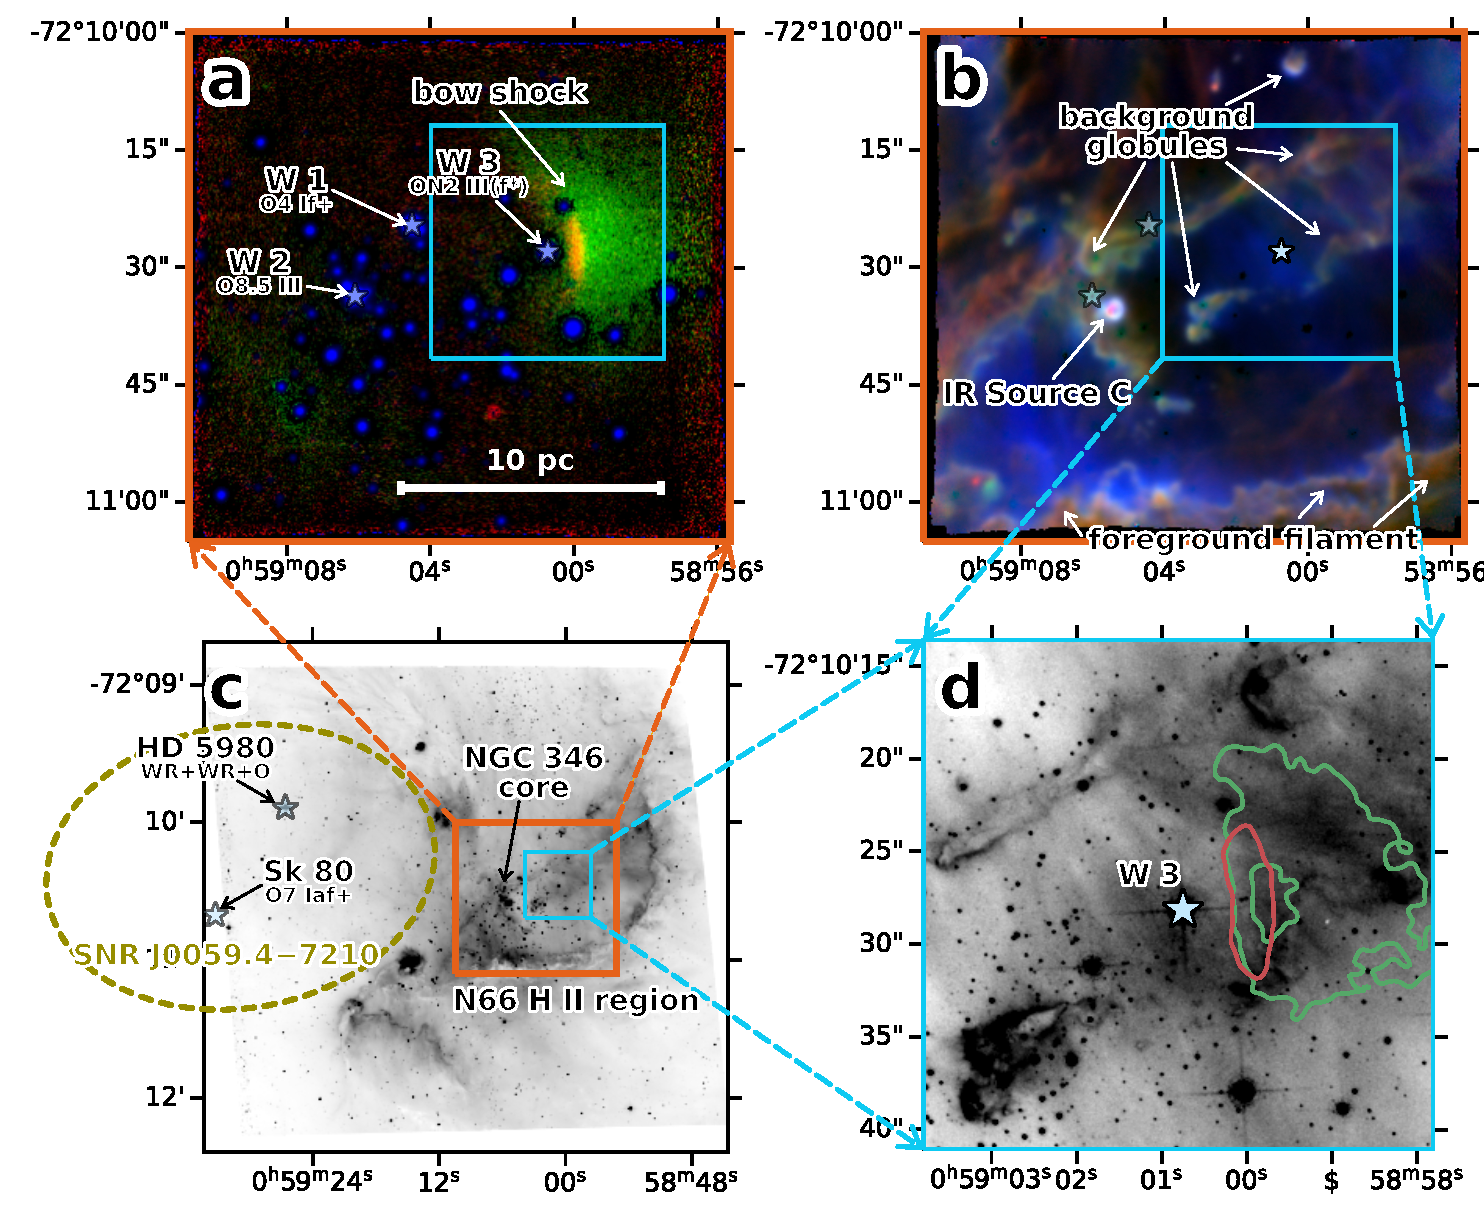
\includegraphics[width=\linewidth]{figs/ngc346-bow-shock-4-panel}
  \caption{
    MUSE emission line images of the core of NGC~346.
    (a)~High-ionization emission from the bow shock.
    Red shows \heii{} \Wav{4686},
    green shows \ariv{} \Wav{4740},
    blue shows continuum emission at \SI{4700}{\angstrom}
    (mainly starlight).
    Star symbols indicate the positions of the most luminous
    ionizing stars in the cluster: Walborn~1, 2, and 3.
    (b)~Medium to low-ionization emission
    from the surrounding N66 \hii{} region.
    Red shows [\ion{O}{1}] \Wav{6300},
    green shows [\ion{S}{2}] \Wav{6731},
    blue shows [\ion{S}{3}] \Wav{9069}.
    (c)~Location of the MUSE field within the wider nebula against
    a background \ha{} image from HST-ACS in the F658N filter.
    The yellow dashed ellipse shows the maximum extent
    of the X-ray emission from the supernova remnant \snrj,
    while star symbols indicate more distant luminous ionizing stars.
    (d)~Zoom of panel~c showing detail of the bow shock region
    in the light of \ha{} emission, with superimposed contours of
    \heii{} (red) and \ariv{} (green). 
    }
  \label{fig:muse-acs-multipanel}
\end{figure*}

\begin{figure*}
  \centering
  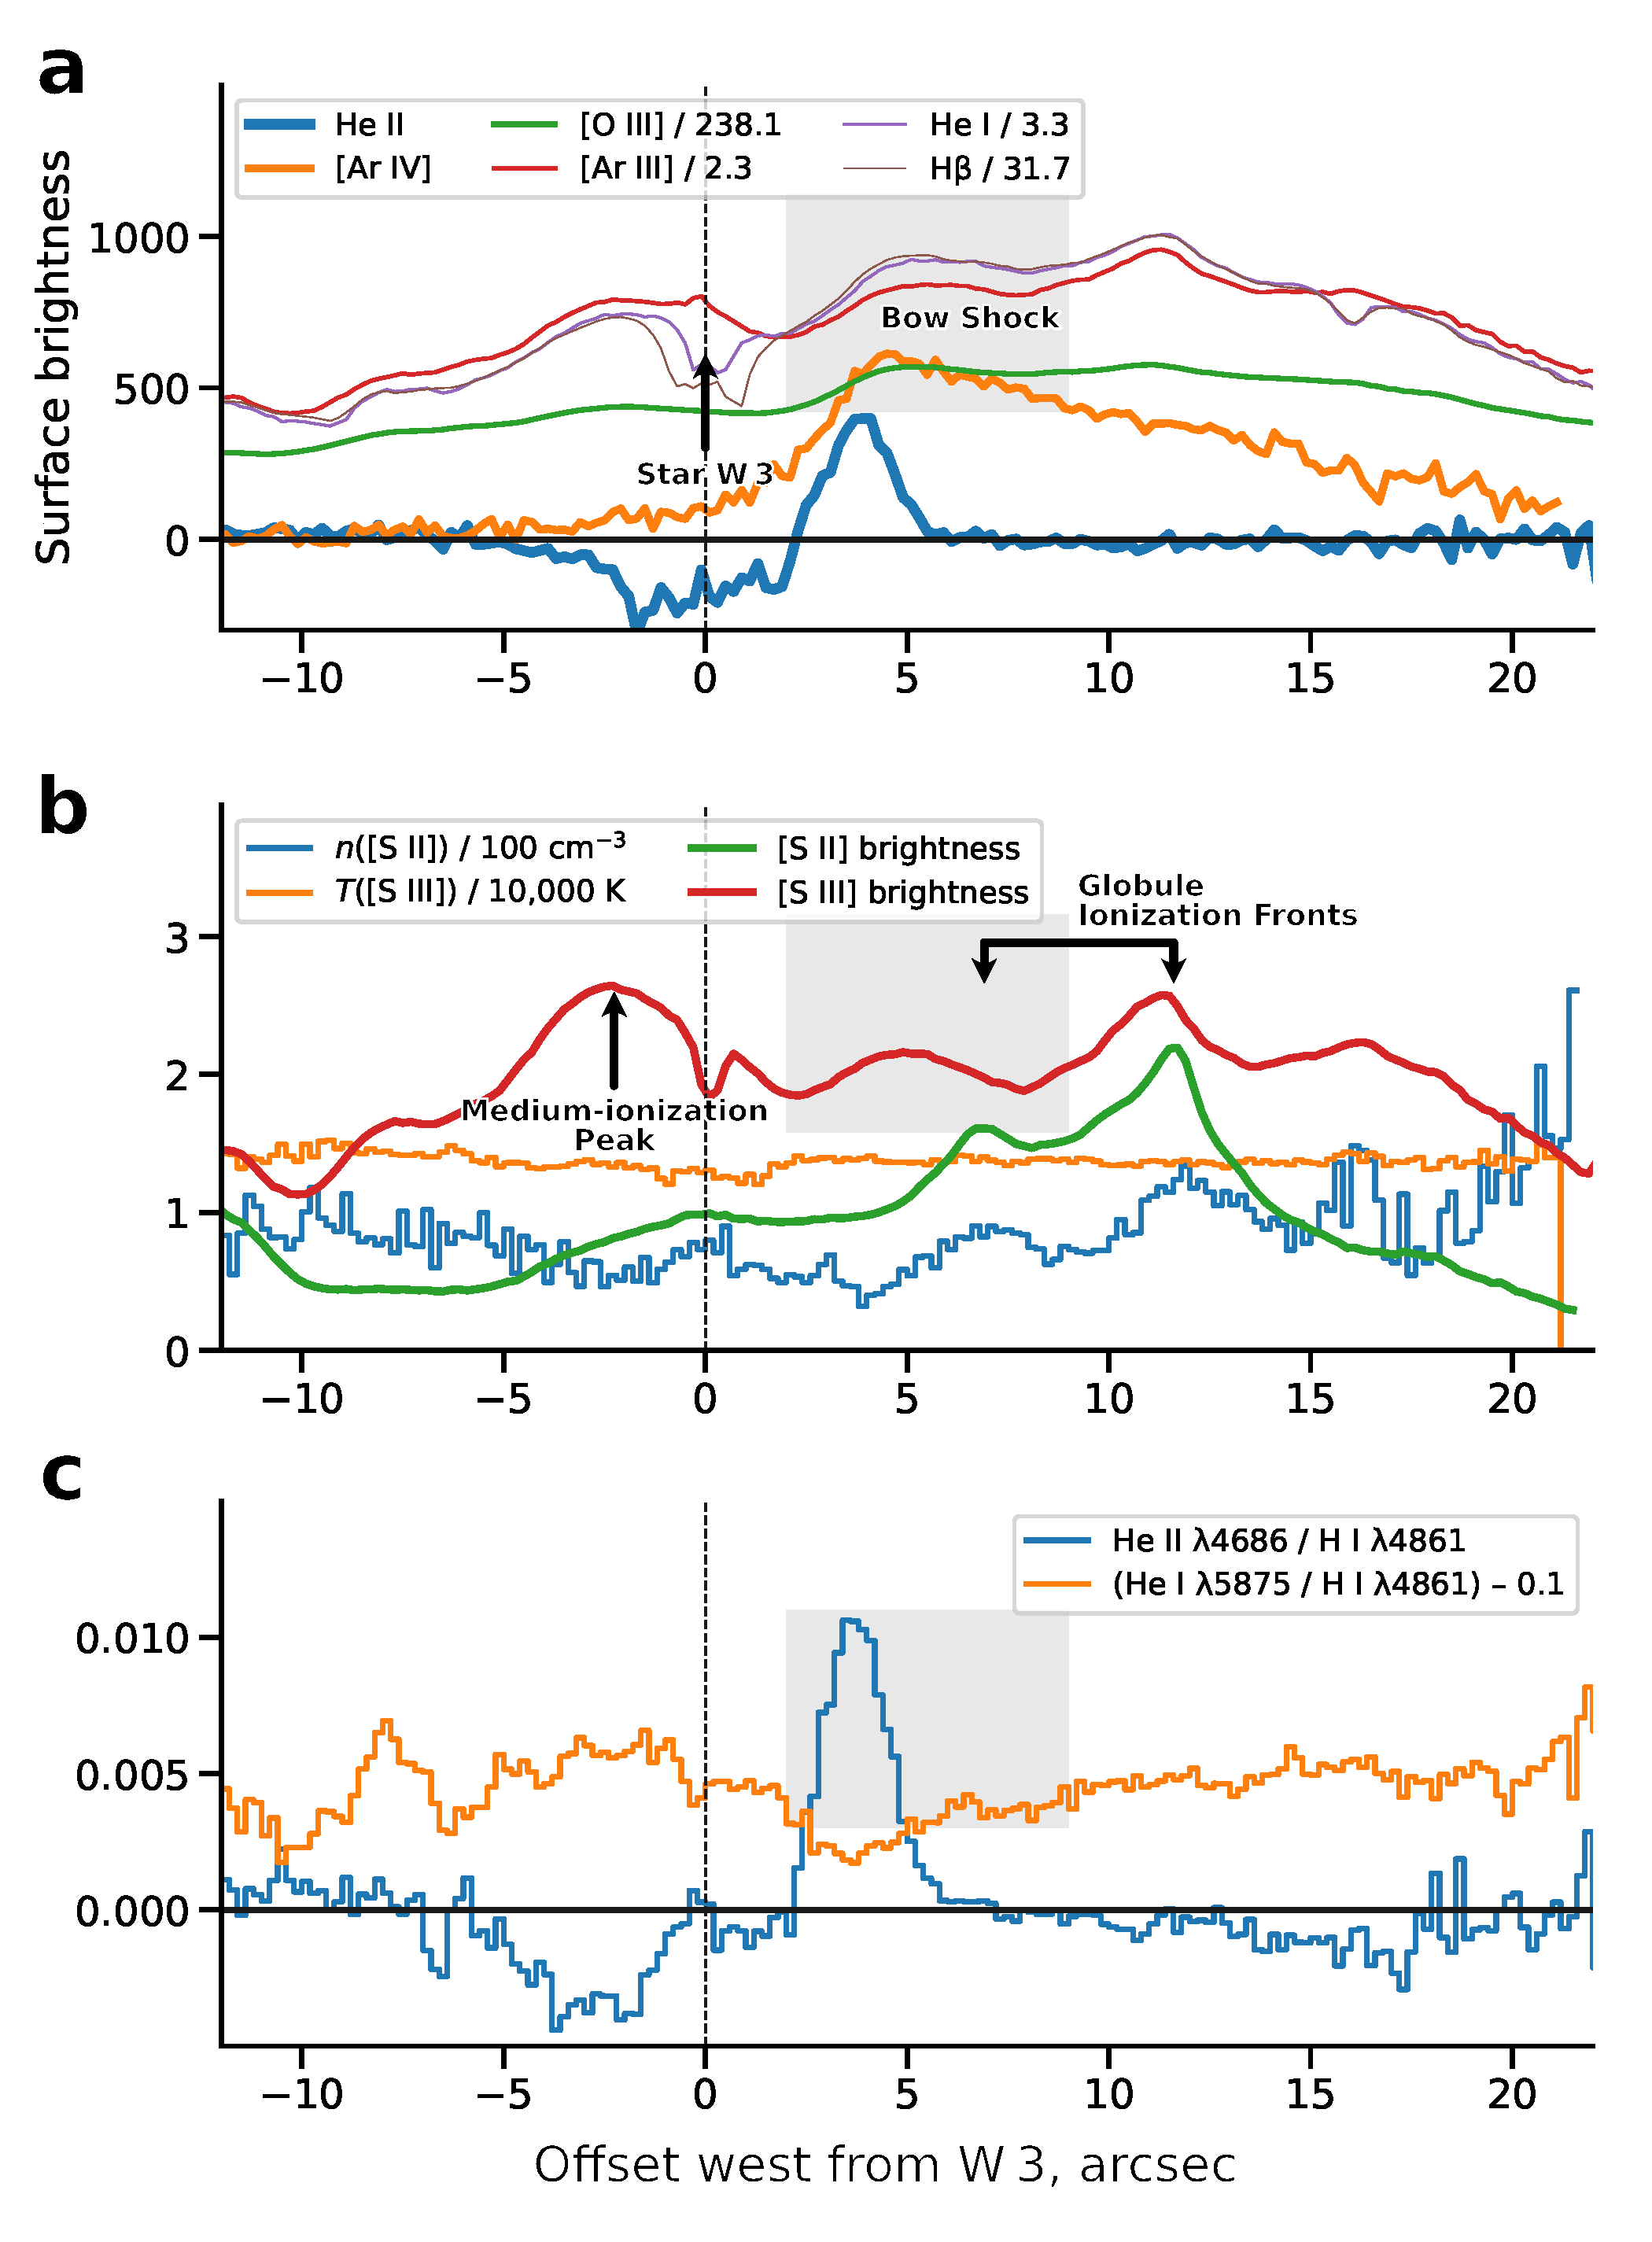
\includegraphics[width=0.9\linewidth]{figs/ngc346-profiles-3-panel}
  \caption{
    (a)~Continuum-subtracted and extinction-corrected
    line surface brightness profiles
    along an East--West cut along the bow shock axis
    of width \SI{4}{arcsec},
    derived from MUSE integral field spectra.
    The gray box indicates the leading edge of the bow shock emission
    for comparison with following figures.     
    Thickest lines show the high ionization emission from
    \heii{} \Wav{4686} (blue) and \ariv{} \Wav{4740} (orange).
    Progressively thinner lines show medium ionization emission from
    \oiii{} \Wav{5007} (green),
    \ariii{} \Wav{7136} (red),
    \hei{} \Wav{5875} (purple), and
    \hb{} \Wav{4861} (brown).
    Vertical scale gives brightness in instrument units,
    for conversion to cgs multiply by
    \SI{1.489e-8}{erg.s^{-1}.cm^{-2}.sr^{-1}}.
    The brightness of medium ionization lines have been scaled
    by factors given in the key, so as to make all the lines
    approximately coincide at the left edge of the gray box.
    (b)~As panel a but showing the \sii{} density (orange)
    and \siii{} temperature (blue), together with
    the brightness profiles of \sii{} \Wav{6731} (red)
    and \sii{} \Wav{9069} (green) on an arbitrary scale.
    (c)~As panel a but showing line ratios of
    \(\heii / \hi\) (blue) and \(\hei / \hi\) (orange).
    A constant value of 0.1 has been subtracted from the latter
    for ease of comparison and to emphasise the slight dip
    in \(\hei / \hi\) at the position of the bow shock. 
    }
  \label{fig:brightness-cuts}
\end{figure*}

The primary observational data set used in this paper
is an archival integral field spectral cube of NGC~346
obtained with the MUSE spectrograph \citep{Bacon:2010a, Bacon:2014a}
on the VLT as part of program 098.D-0211(A) (PI:  W.-R. Hamann). 
The usable field of view is approximately
\SI{64}{arcsec} times \SI{60}{arcsec} with
spaxel size of \SI{0.2}{arcsec} and estimated seeing
full-width half maximum (FWHM) width of \SI{0.961}{arcsec}.
The spectral range is \SI{4595}{\angstrom} to \SI{9366}{\angstrom}
sampled at \SI{1.25}{\angstrom.pix^{-1}} and the
spectral resolving power varies from \(R \approx 2000\) in the blue
to \(R \approx 4000\) in the red.
We use reduced data from the standard ESO pipeline processing
\citep{Weilbacher:2020a},
co-added across multiple observations obtained on \mbox{2016-08-22}
with a total effective exposure time of \SI{12600}{s}.

We divide the spectral range into sections of width \SI{800}{\angstrom}
and fit a 6th order polynomial to the continuum
in line-free wavelengths of each section,
using an independent fit for each spaxel.
We then extract individual emission lines (or close blends)
from the continuum-subtracted spectra using \SI{5}{\angstrom} windows,
centered on the expected wavelength of each line
in the systemic frame of the nebula
(heliocentric velocity \(V \approx \SI{+160}{km.s^{-1}}\)).
We correct for an over-subtraction of the sky background,
which is apparent in the pipeline-processed data cube.
We establish accurate zero points for all lines by checking that
multiple line ratios tend towards physically reasonable asymptotes
as the brightness tends towards zero.

We use the observed Balmer decrement between \ha{} and \hb{} to
correct all lines for foreground dust extinction, assuming
an SMC-appropriate reddening law with \(R_V = 2.74\)
\citep{Fitzpatrick:1990a, Gordon:2003l}.
The reddening is low over most of the field
(\(E(B - V) \approx 0.1\))
but reaches \(E(B - V) \approx 1\) along the southern edge
(labeled ``foreground filament'' in
Figure~\ref{fig:muse-acs-multipanel}b).


\section{Results}
\label{sec:results}

An east-facing bow shock structure is detected
around the star Walborn~3,
as illustrated in Figure~\ref{fig:muse-acs-multipanel}a.
The inner edge of the bow shock is traced
by a sharp ridge of \heii{} \Wav{4686} emission (red),
while \ariv{} \Wav{4740} emission (green)
is more extended with a diffuse outer boundary. 
Nebular emission of the same field in moderate
and low ionization lines is shown in
Figure~\ref{fig:muse-acs-multipanel}b and
there is no evidence of the bow shock in these lines.
Instead, the low ionization lines
([\ion{O}{1}], red, and [\ion{S}{2}], green)
trace the ionization fronts at the surface
of dense filaments and globules,
while the moderate ionization line ([\ion{S}{3}], blue)
traces diffuse ionized gas in the interior of
the nebula that is largely unrelated to the bow shock. 

Figure~\ref{fig:muse-acs-multipanel}c shows the
position of the MUSE field (orange box) on a wider scale
\textit{HST} image of the N66 \hii{} region
\citep{Nota:2006x}.
The head of the bow shock is oriented towards
the bright N--S oriented filament that is located
outside of the MUSE field to the West,
and which represents a large scale ionization front
at the edge of the \hii{} region.
The supernova remnant \snrj{} is centered roughly
\SI{1}{arcmin} to the East of the \hii{} region,
but based on the X ray emission \citep{Maggi:2019q}
it does not overlap the MUSE field. 

Figure~\ref{fig:muse-acs-multipanel}d shows a zoomed view of
the \textit{HST} \ha{} image around W~3, compared
with contours of the bow shock emission.
The \ha{} brightness does appear to be slightly higher
within the bow shock contours than just outside it,
but the effect is very subtle compared with the
general fluctuations in \ha{} brightness in the nebula.

Figure~\ref{fig:brightness-cuts}a shows surface brightness
profiles in multiple emission lines along an East--West
cut along the bow shock axis.
The \heii{} emission peak lies at an offset \SI{4}{arcsec}
west from the star W~3, with a width (FWHM) of about \SI{2}{arcsec}
(note that \(\SI{1}{arcsec} \approx \SI{0.3}{pc}\)
at the distance of the SMC). 
The \heii{} brightness becomes negative close to the
star position due to contamination by the photospheric
absorption line.
The \ariv{} emission peak lies slightly farther from the star
(\SI{4.5}{arcsec}) and shows a gradual linear decline with
\(\text{FWHM} \approx \SI{20}{arcsec}\).
In both lines, diffuse nebular emission is undetectably small 
in the region around the bow shock.
The moderate ionization lines, on the other hand, are dominated
by the large-scale nebular emission and vary by a factor of only
\num{1.5} to \num{2} along the entire slit.
Nonetheless, there is an apparent rise in the brightness
of these lines at the position of the bow shock
(see gray box in Figure)
that tracks the rise and fall of the \ariv{} line.
This increase amounts to about 50\% of the diffuse nebular emission
in the case of \oiii{} and the H and He recombination lines
and about 30\% in the case of \ariii{}.

Figure~\ref{fig:brightness-cuts}b shows density and temperature
diagnostics


\begin{figure}
  \centering
  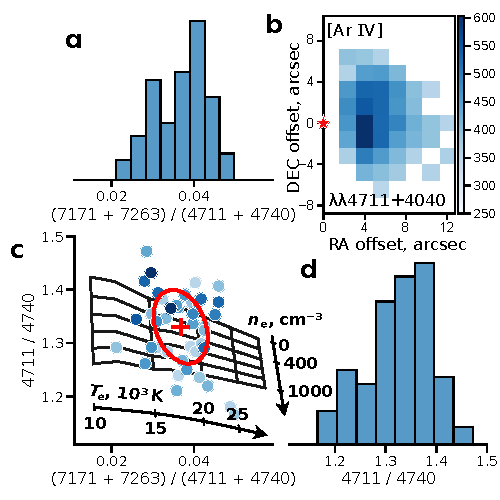
\includegraphics[width=\linewidth]{figs/ngc346-bow-shock-ariv-diagnostics-annotated}
  \caption{
    Temperature and density diagnostics of the bow shock from \ariv{} line ratios.
    }
  \label{fig:ariv-diagnostics}
\end{figure}


\section{Longslit observations}
\label{sec:longsl-observ}
\begin{figure*}[p]
  \centering
  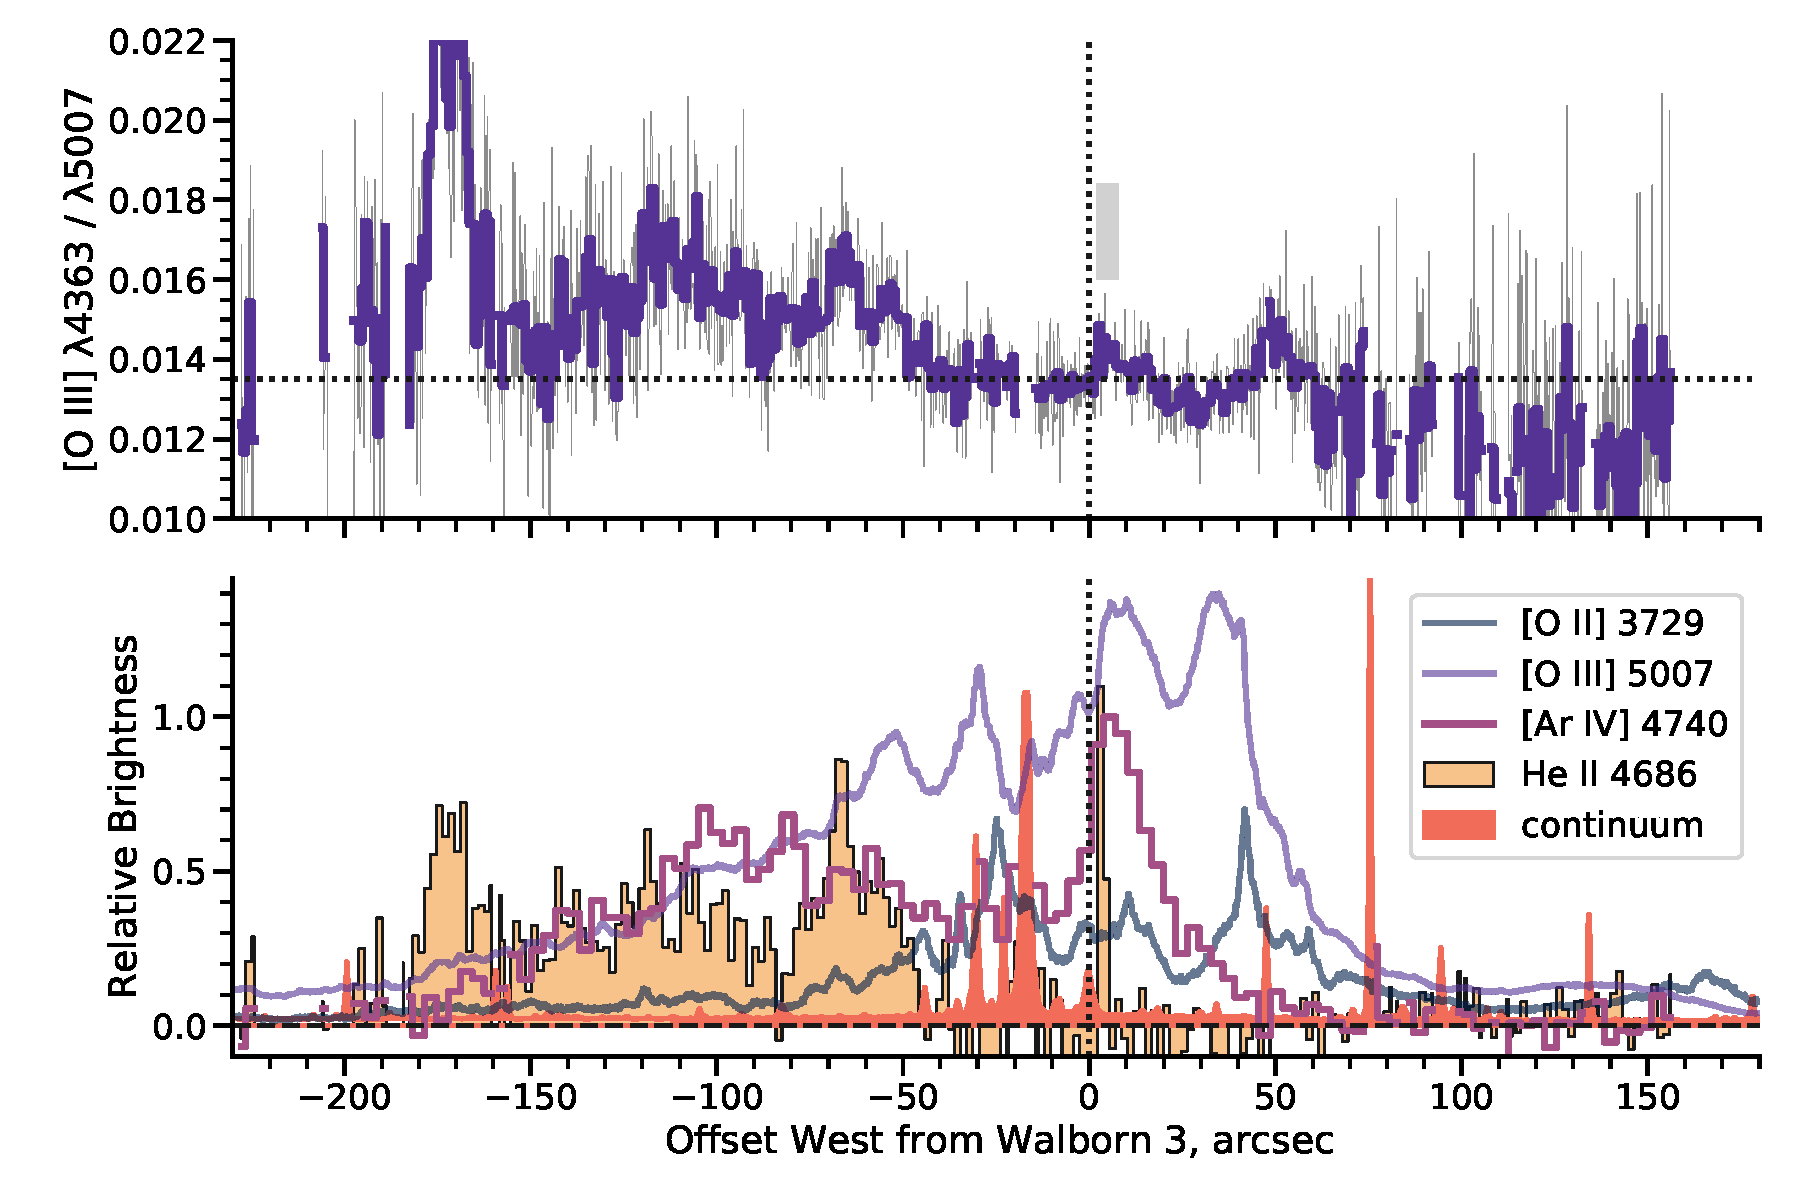
\includegraphics[width=0.9\linewidth]{figs/ngc346-fors1-combo}
  \caption{
    Emission line surface brightness profiles and line ratios along a large-scale
    East--West cut across the entire region, based on FORS1 longslit spectra.
    The slit is close to the symmetry axis of the bow shock.
    (a) Temperature-sensitive line ratio \oiii{} 4363/5007.
    The gray box shows the same inner rim region of the bow shock
    that is highlighted by a gray box in Fig.~\ref{fig:brightness-cuts}.
    (b) Selected emission lines from a wide range of ionization stages. 
    }
  \label{fig:oiii-ratio}
\end{figure*}

\begin{figure}
  \centering
  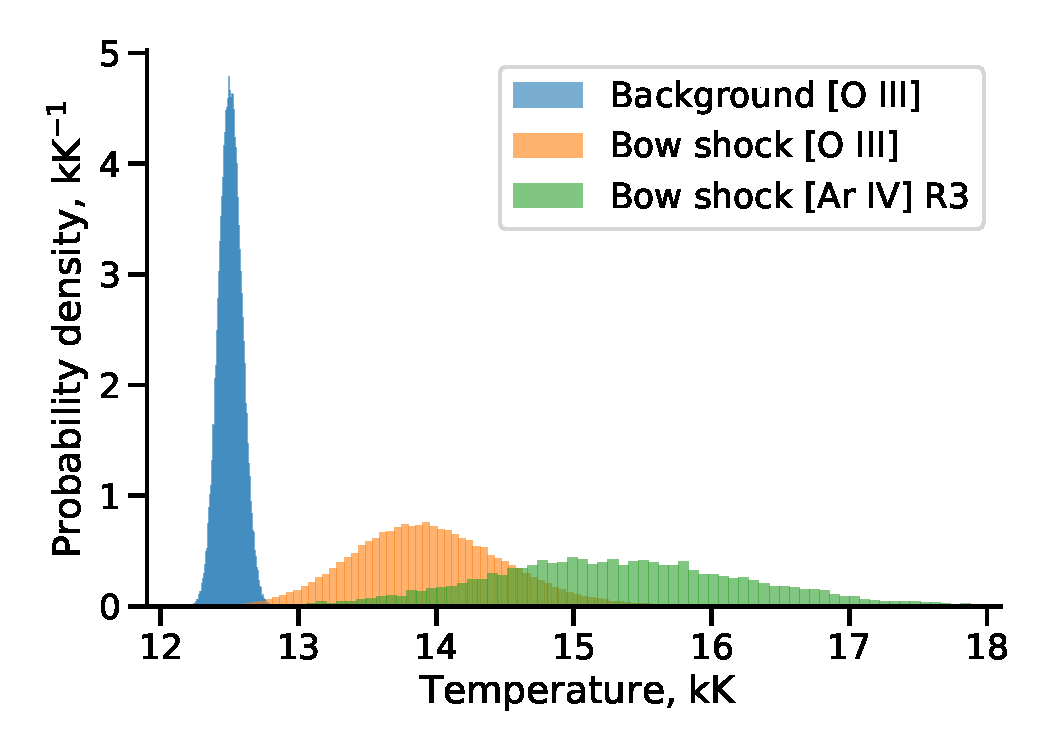
\includegraphics[width=\linewidth]{figs/ngc346-bowshock-T-oiii-ariv}
  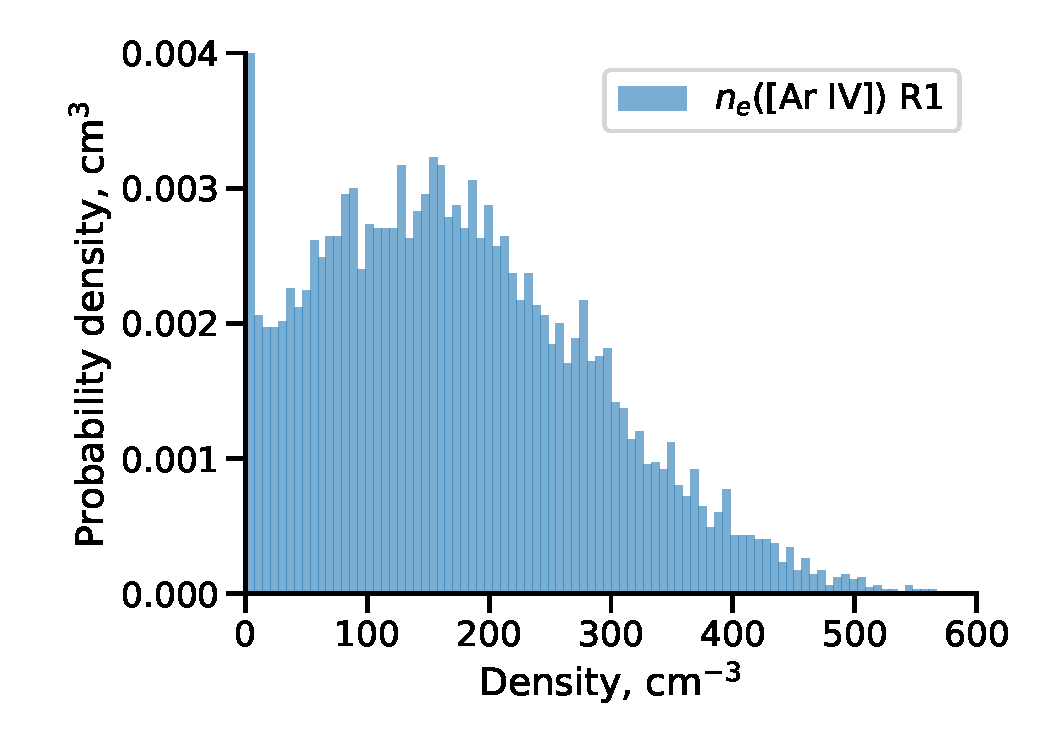
\includegraphics[width=\linewidth]{figs/ngc346-bowshock-den-ariv}
  \caption{
    Derived temperature of nebula and bow shock
    from FORS longslit observations.
    }
  \label{fig:T-oiii-ariv}
\end{figure}




Apart from the inner rim of the bow shock,
there is no diffuse \heii{} emission in the core of NGC~346,
or in the western side of the N66 region.
The eastern side of N66, on the other hand,
shows extensive \heii{} \Wav{4686} emission,
as can be seen at offsets from \num{-200} to \SI{-50}{arcsec}
in Figure~\ref{fig:oiii-ratio}b.
The eastern side of N66 also shows a ten times higher [\ion{Fe}{3}] / \hb{} ratio
and disturbed kinematics in low-ionization lines such as \sii{}.
All these are probably due to a foreground supernova remnant SNR~B0057\(-72.2\) \citep{Ye:1991d}
that overlaps with this part of the nebula \citep{Chu:1988m, Naze:2002q, Danforth:2003m, Maggi:2019q, Matsuura:2022v}.


\section{Mid-infrared emission}
\label{sec:mid-infr-emiss}


\begin{figure*}
  \centering
  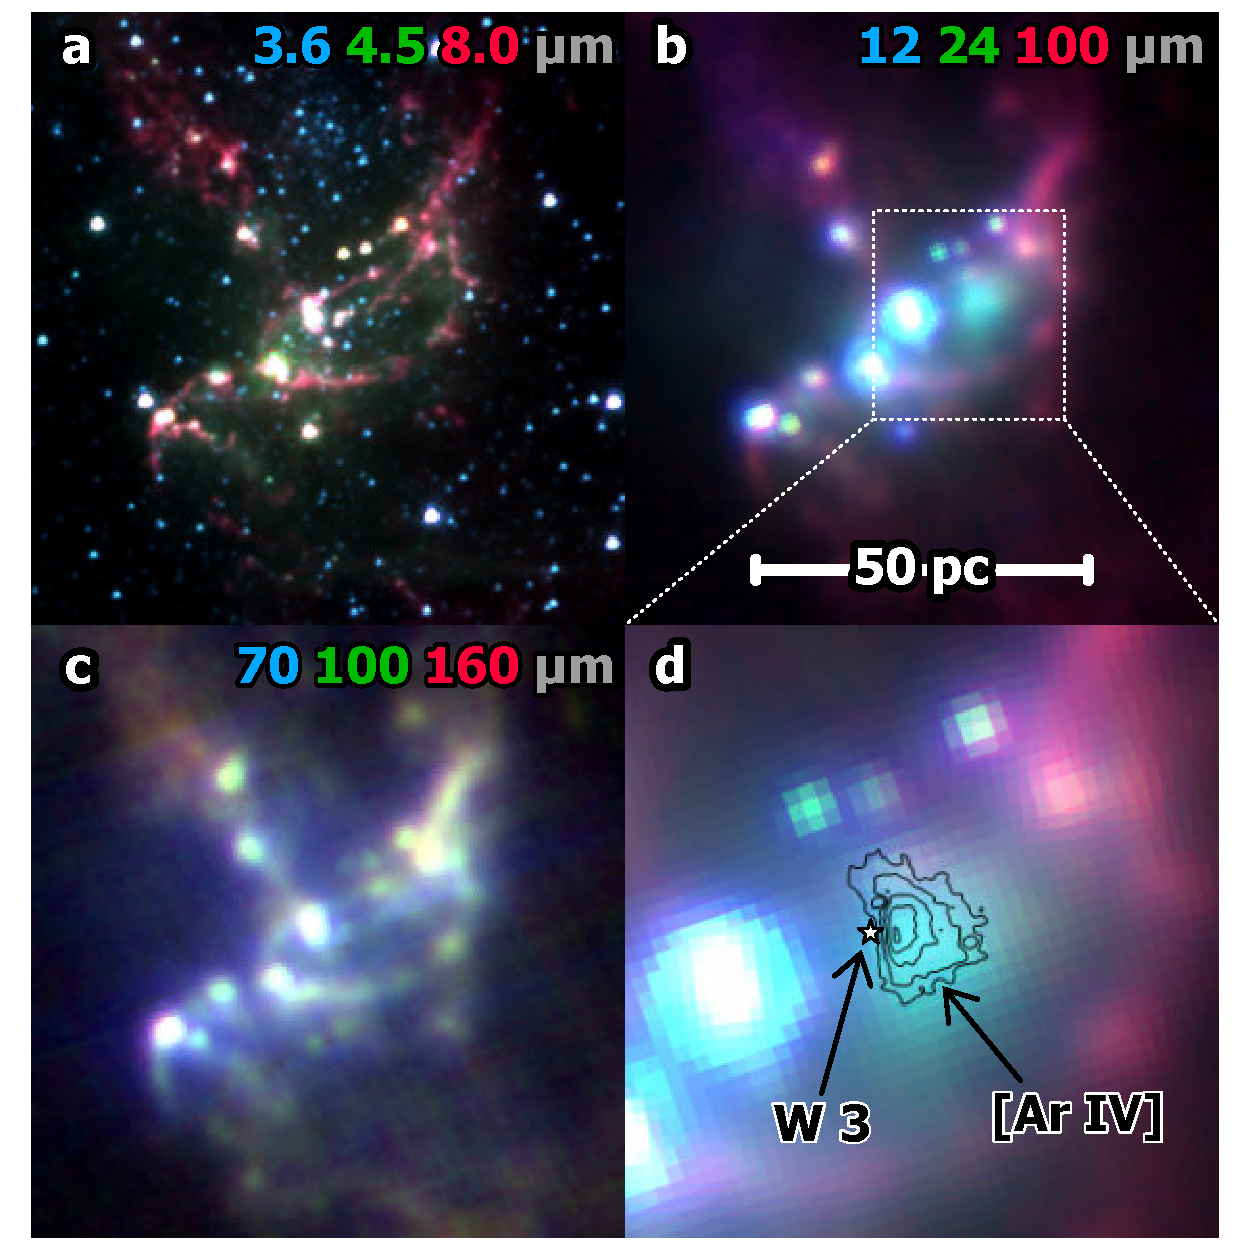
\includegraphics[width=\linewidth]{figs/ngc346-infrared-multipanel}
  \caption{
    Panoramic view of the NGC~346/N66 region at infrared wavelengths:
    (a)~Short wavelength mid-infrared (\num{3.6} to \SI{8}{\um});
    (b)~Longer wavelength mid-infrared (\num{12} to \SI{100}{\um});
    (c)~Far-infrared (\num{70} to \SI{150}{\um});
    (d)~Zoomed view of panel~b.
    Images are from satellite observatories as follows:
    \textit{Spitzer} IRAC \num{3.6}, \num{4.5}, \SI{8}{\um});
    \textit{WISE} \SI{12}{\um};
    \textit{Spitzer} MIPS \num{24}, \SI{70}{\um};
    \textit{Herschel} PACS \num{100}, \SI{150}{\um}.
    }
  \label{fig:infrared-multipanel}
\end{figure*}
\begin{figure}
  \centering
  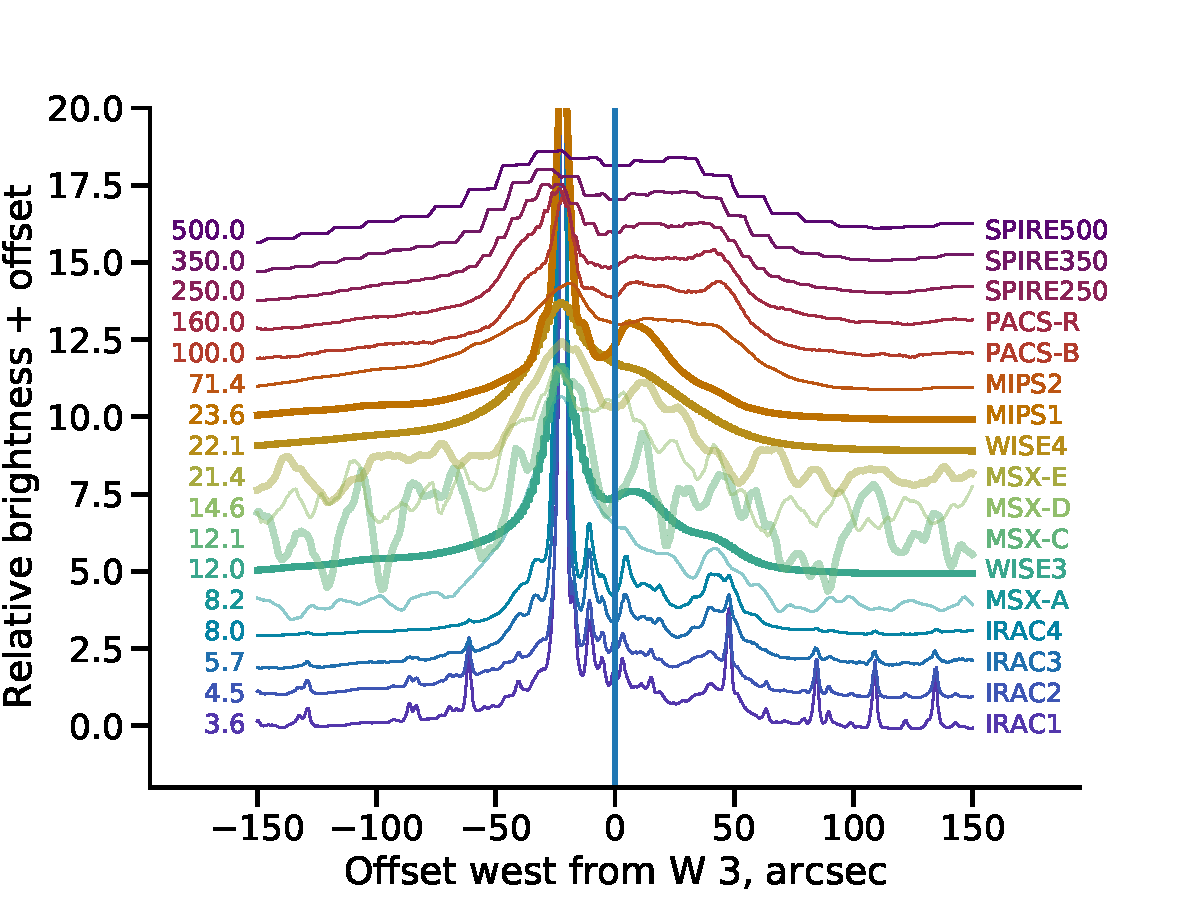
\includegraphics[width=\linewidth]{figs/ngc346-infrared-profiles}
  \caption{
    East--west brightness profile cuts in various infrared bands. 
    }
  \label{fig:infrared-profiles}
\end{figure}

\begin{figure}
  \centering
  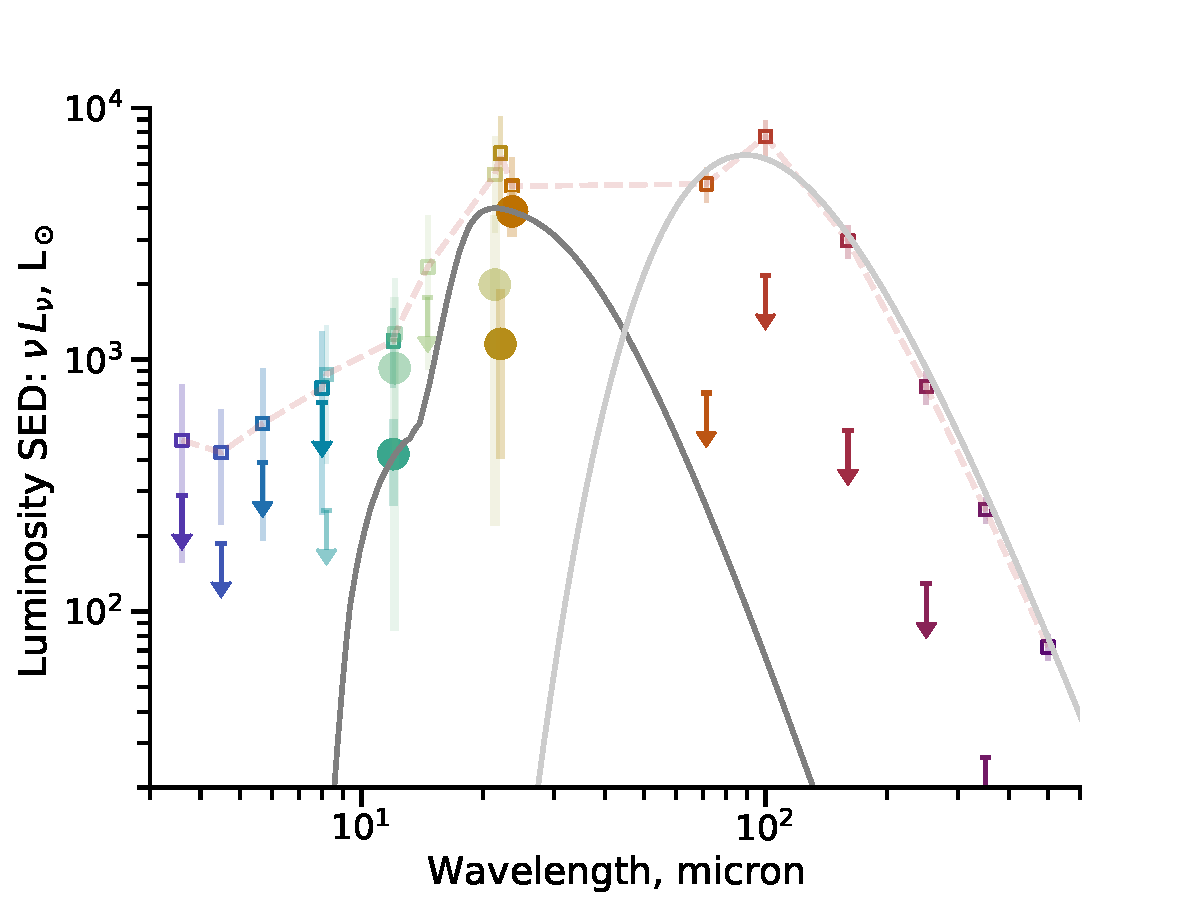
\includegraphics[width=\linewidth]{figs/ngc346-infrared-sed}
  \caption{
    Spectral energy distribution of bow shock (large symbols and downward arrows)
    and background nebula small symbols joined by dashed line.
    }
  \label{fig:infrared-sed}
\end{figure}







\section{Discussion}
\label{sec:discussion}

Is there any possibility it might be a runaway?

What is the reason that we detect this bow shock
at optical wavelengths, which is not typical?
Probably due to the presence of the high ionization stages,
which allow the weak bow shock emission to be
separated from the background hii region.
This is similar to the argument of \citep{Danforth:2003m}
as to why it is better to use UV observations to find SNR in
bright hii regions. 


\section{Conclusions}
\label{sec:conclusions}

\begin{acknowledgments}
  Thank you.
\end{acknowledgments}

\facilities{VLT:Yepun (MUSE)}

\bibliography{smc-bow-refs}

\end{document}

%%% Local Variables:
%%% mode: latex
%%% TeX-master: t
%%% End:
